\chapter{Driving on the ground state manifold}
Of special importance in theory of the ground state manifold are geodesics. It is not yet clear what role they have in general, but in some special cases its well known, see \cite{polkovnikov}. The holy grail of this theory would be to find path with the lowest excitation amplitude, which is not an easy task.

Let's have a geodesic $\mathcal{G}(t)$ and some curve $\gamma(t)$ on the ground stat manifold, spanning between points $P_i$ and $P_f$ during some time $t_f$, meaning
 $$\mathcal{G}(0)=\gamma(0)=P_i\in\mathcal{M}_0,\qquad \mathcal{G}(t_f)=\gamma(t_f)=P_f\in\mathcal{M}_0.$$

Excitation amplitude during infinitesimal quench is $\d s$, therefore $\sum_i \Delta s_i$ summed along path $\gamma(t)$ is the amplitude of transport along that path. This can be more rigorously expressed by functional
\begin{equation}
    s_\gamma=\int_{\gamma(t)}\d s=\int_{0}^{t_f}\sqrt{g_{\mu\nu}\dot\lambda^\mu\dot\lambda^\nu}\d t
\end{equation}
This is the entity, which is minimal if $\gamma$ is a geodesic. Before moving on, lets quickly review the proof of this statement.

\begin{proof}[Geodesics minimize the distance on manifold]
    Functional of distance is
    \begin{equation}
        s=\int\mathcal{L}(t,\lambda^\mu,\dot\lambda^\mu)\d t
    \end{equation}
    for 
    \begin{equation}
        \mathcal{L}=\sqrt{g_{\mu\nu}\dot\lambda^\mu\dot\lambda^\nu}.
    \end{equation}
    Using Euler-Lagrange equations 
    \begin{equation}
        \der{\mathcal{L}}{\lambda^\mu}-\der{}{t}\der{\mathcal{L}}{\dot\lambda^\mu}=0,
    \end{equation}
    we get for $g_{\mu\nu}=g_{\mu\nu}(\lambda^\mu)$ second order differential equation
    \begin{equation}
        \ddot\lambda^\mu+\Gamma^\mu_{\;\;\alpha\beta}\dot\lambda^\alpha\dot\lambda^\beta=0\qquad \Gamma^\mu_{\;\;\alpha\beta}=\frac{1}{2}g^{\mu\kappa}\left(g_{\kappa\alpha,\beta}+g_{\kappa\beta,\alpha}-g_{\beta\alpha,\kappa}\right),
        \label{eq:geodesicEquaiton}
    \end{equation}
    which is the Geodesic equation.
\end{proof}

Excitation probability along the path $\gamma$ can be formally written as $F=\sum_i\Delta s_i^2$, which cannot be simply calculated as $s^2$. Because $\Delta s_i>0$, we have
\begin{equation}
    \begin{split}
        \sum_i \Delta s_i^2& <(\sum_i\Delta s_i)^2\\
        F&<s^2.
    \end{split}
\end{equation}

This doesn't necessarily mean, that fidelity along geodesic will be minimal ($F(\mathcal{G})<F(\gamma)$), because we didn't rule out the scenario 
$$F(\gamma)<F(\mathcal{G})<s_\mathcal{G}^2<s_\gamma^2.$$

This means, that the geodesic equation cannot be used for fidelity minimization and some new insight is needed. The functional, which needs to be minimized is
\begin{equation}
    F=\int\int g_{\mu\nu}\d\lambda^\mu\d\lambda^\nu = \int_{t_i}^{t_f}\underbrace{\int_{t_i}^\tau g_{\mu\nu}\der{\lambda^\mu}{t}\der{\lambda^\nu}{t} \d t}_{\mathcal{L}(\lambda^\mu,\dot\lambda^\mu,\tau)}\d \tau .
\end{equation}
Using Euler-Lagrange equations, again for time independent $g_{\mu\nu}=g_{\mu\nu}(\lambda^\mu)$, leads to
\begin{equation}
    \int_{t_i}^{t_f}\left[g_{\mu\nu,\kappa}\dot\lambda^\mu\dot\lambda^\nu - \der{}{t}\left[g_{\mu\nu}\left(\delta^\mu_\kappa\dot\lambda^\mu+\dot\lambda^\mu\delta^\nu_\kappa\right)\right]\right]\d t=0
\end{equation}
which needs to be zero for integration over any subset $(t_i,t_f)$ leading to zero condition for the integrand itself, which leads to geodesic equation \ref{eq:geodesicEquaiton}, as in the case of distance on manifold.



\textcolor{blue}{Polkovnikov for some special case: They play a role of "maximum fidelity at any time" transport, meaning at any given time $t$ the fidelity on corresponding point on geodesics will be less than of $\gamma$
$$F(\mathcal{G}(t))<F(\gamma(t)).$$ }









\section{The role of geodesics}


\subsection{Minimizing the energy variance}
From \cite{Bukov2019}.
About transports using \emph{fast forward} Hamiltonian means the system is driven to the target state in some fixed amount of time. The transport is done on the ground state manifold $\M$.

\conjecture{
    For any fast forward Hamiltonian $\HH(\lambda(t))$ driven along one dimentional path $\lambda(t): \R\mapsto \R$ using time $t$ as parametrization, the energy fluctuations $\delta E^2$, averaged along the path, are larger than the geodesic length $l_\lambda$
    \begin{equation}
        \int\limits_0^T\sqrt{\delta E^2(t)}\d t \eqqcolon l_t\geq l_\lambda \int\limits_{\lambda_i}^{\lambda_f} \sqrt{g_{\lambda\lambda}} \d \lambda=\int_0^T \sqrt{g_{\lambda\lambda}}\frac{\d \lambda}{\d t}\d t.
    \end{equation}
    The length $l_\llambda$ is defined in control space (with metric tensor $g_{\lambda\lambda}$) and is generally larger than the distance between wave functions, i.e. the absolute geodesic (defined with $G_{\mu\nu}$). From its definition, we can see that it corresponds to the metric tensor as we use it.
    
    
    
    The energy variance is 
    \begin{equation}
        \delta E^2= \braket{o(t)|\HH(t)^2|o(t)}-\braket{o(t)|\HH(t)|o(t)}^2=\braket{\partial_t (t)|\partial_t o(t)})_c=G_{tt}
    \end{equation}    
    and the Metric tensor in control space is defined as
    \begin{equation}
        g_{\lambda\lambda}\coloneqq \braket{\partial_\lambda o(t)|\partial_\lambda o(t)})_c
    \end{equation}
}


\begin{proof}
    \begin{equation}
        \delta E^2\equiv \braket{o(t)|\HH(t)^2|o(t)}_c=\dot\lambda^2 G_{\lambda\lambda}+\O(\dot\lambda^4),
    \end{equation}
    where $\O(\dot\lambda^4)$ needs to be positive for any real-valued Hamiltonian. This comes from the fact, that it has instantaneous time-reversal symmetry.
\end{proof}

The conjecture only applies to unit fidelity protocols ($F(t)=1 \;\forall t\in[0,T_f]$) and can be extended to an arbitrary dimensional path.












\section{The meaning of geodesics}


\subsection{Transport using quenches}
\label{sec:quenches}
Unifying the ground states $\ket{o(\llambda)}$ over all points $\llambda\in\R^n$ in the parameter space, we get the ground state manifold. Here the fidelity $f$ and distance $s$ are defined
\begin{equation}
    \d s^2 \equiv 1-f^2\equiv 1-\left|\braket{o(\bm\llambda+\delta\bm\llambda)|o(\bm\llambda)}\right|^2.
    \label{eq:distanceOnM0}
\end{equation}

The final fidelity of transport on $\M$ is then
\begin{equation}
    F=\iint g_{\mu\nu}\d\lambda^\mu\d\lambda^\nu = \int_{t_i}^{t_f}\underbrace{\int_{t_i}^\tau g_{\mu\nu}\der{\lambda^\mu}{t}\der{\lambda^\nu}{t} \d t}_{\mathcal{L}(\lambda^\mu,\dot\lambda^\mu,\tau)}\d \tau .
\end{equation}
Using Euler-Lagrange equations for time-independent $g_{\mu\nu}=g_{\mu\nu}(\lambda^\mu)$, leads to
\begin{equation}
    \int_{t_i}^{\tau}\left[g_{\mu\nu,\kappa}\dot\lambda^\mu\dot\lambda^\nu - \der{}{t}\left[g_{\mu\nu}\left(\delta^\mu_\kappa\dot\lambda^\nu+\dot\lambda^\mu\delta^\nu_\kappa\right)\right]\right]\d t=0,
\end{equation}
which needs to be zero for integration over any subset $(t_i,\tau)$. This can bne achieved for any path only it the integrand itself is zero, which happens if the geodesic equation holds.

The fidelity $f$ measures transition probability between two neighboring eigenstates of two different Hamiltonians. Those two states belong to the same Fibre space $\PH(\llambda)\times \R^n$ from which the coefficients $(\Z,\llambda)$ are taken. Because all $\PH(\llambda)$ are canonically isomorphic, there is no problem in parallel transport from one space to another, which is needed for braket\footnote{This procedure is done without thinking in the back part of our brains such, that we don't even think about it. That's how trivial it is.}.

The distance minimization runs into some interpretation problems. On one hand, minimalization of the distance is equivalent to maximalization of the sum of infinitezimal fidelities along the path (we say we \emph{maximize the fidelity along the path}). On the other hand we are using only ground states in every step of the transport, therefore defining the fidelity to be one. There are actually two ways out of this confusion. \emph{Perturbed adiabatic driving} and \emph{Transport using quenches}.


\subsubsection{Perturbed adiabatic driving}
It the first case, we imagine at every point of transport, that the fidelity is small enough, such that in eigenbasis and some small parameters $\delta_i\in \mathbb{C}$ we get
$$\ket{o(\llambda_i)}\equiv \begin{pmatrix}
    Z_0(\llambda_i)\\
    0\\
    \vdots \\
    0
\end{pmatrix} \overset{\text{transport }\d s}{\longrightarrow} \ket{o(\llambda_i+\delta \llambda)}\equiv\begin{pmatrix}
    Z_0(\llambda_i+\delta \llambda)\\
    0\\
    \vdots \\
    0
\end{pmatrix} +\underbrace{\begin{pmatrix}
    0\\
    \delta_1(\llambda_i+\delta \llambda)\\
    \vdots \\
    \delta_n(\llambda_i+\delta \llambda)
\end{pmatrix}}_{\mathbf{\Delta}(\llambda_i+\delta \llambda)}, $$
where the last term is neglected using 
$$\braket{\Delta(\llambda)|o(\llambda+\delta\llambda)}\approx 0.$$

This might have interesting implication for slow transports, or small distance transports. For example when some slow thermalization is considered during a transport.









\section{Transport using quenches}
If we imagine $\delta\llambda$ to be finite (not infinitely small, as the notation suggests), the \textbf{transport} means \textbf{doing a sequence of quenches and measuring the system after every quench}.


Some notion of the space of our Hamiltonian can be seen by quenching from $(\lambda_i;\chi_i)=(0;0)$ to $(\lambda;\chi)$, as can be seen in Figure \ref{fig:quenchFidelityFrom00}.

In Figure \ref{fig:equidistantPointsOnPath} are marked equidistant points, meaning $\int_a^b \d s=\text{const.}$ between every two neighboring points on curve. This means that if the system is measured periodically, the quenches jump smaller distances when closer to a singularity.

Decreasing time step $\Delta t$ has no effect on the relative fidelity of quenches during the evolution but has an effect on their magnitude. As one would expect from \emph{quantum Zeno effect}, when $\Delta t\rightarrow 0$, the transport becomes adiabatic, and the fidelity at any time will become 1. This can be observed in Figure \ref{fig:plotsFidelityQuenches}, such that the shape of the point-like paths looks similar in the columns, and their magnitude decreases.

The quantum Zeno effect for this case can be shown dirrectly by splitting the distance $s$ to $N$ equal pieces. The fidelity for $N$ splits will then be
\begin{equation}
    f(N)=(1-\Delta s)^N=\left(1-\left(\frac{s}{N}\right)^2\right)^N \;\;\overset{N\rightarrow\infty}{\longrightarrow}\;\; 1,
\end{equation}
meaning the consequent measurements will colapse the system to its instantenous eigenstate and the adiabatic condition for transport holds. 

Such measurements can be achieved by fast thermalization of the system. If the finite speed thermalization with $N=T/\tau$ for the mean time between two measurements $\tau$, we get
\begin{equation}
    \begin{split}
        \log f(N) &= N \log \left(1-\left(\frac{s}{N}\right)^2\right) = -\frac{s^2}{N}+o\left(\frac{s^4}{n^3}\right)\\
        f(N) &= \exp\left(-s^2\frac{\tau}{T}-\frac{s^4}{2 N^3}\dots\right) = \exp\left(-s^2\frac{\tau}{T}\right)\left(1+o\left(\frac{s^4}{N^3}\right)\right)
    \end{split}
\end{equation}


\begin{figure}[H]
    \centering
    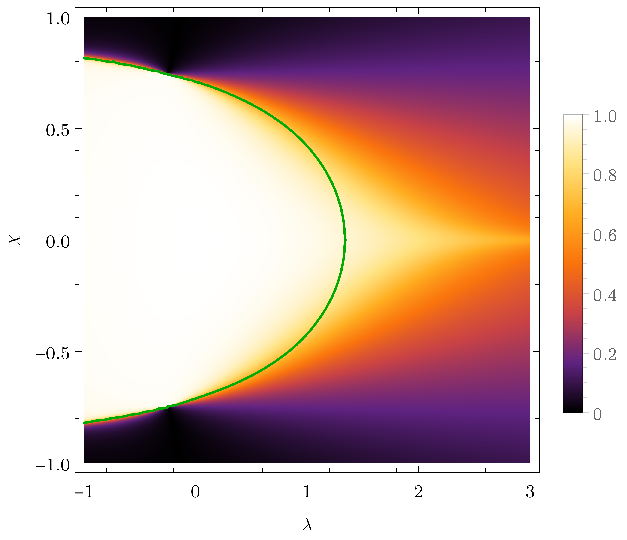
\includegraphics[scale=1.2]{../img/quenchFidelityFrom00.pdf}
    \caption{Arctangens of the fidelity of quenches from $(\lambda_i;\chi_i)=(0;0)$ to $(\lambda;\chi)$.}
    \label{fig:quenchFidelityFrom00}    
\end{figure}

\begin{figure}[H]
    \centering
    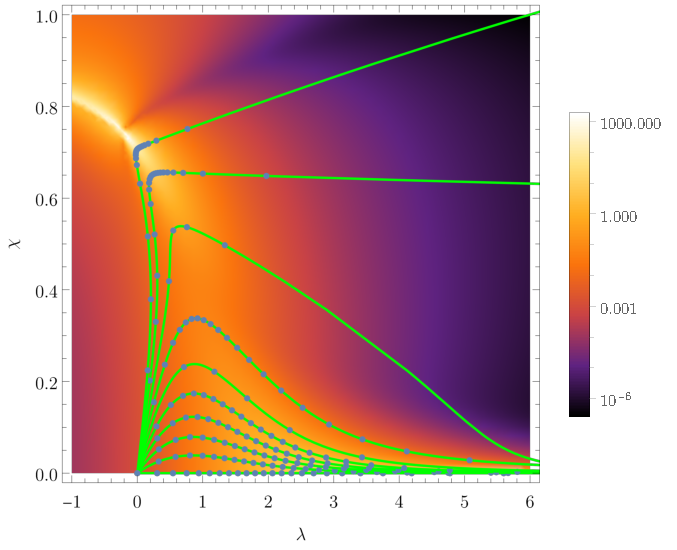
\includegraphics[scale=1.2]{../img/equidistantPointsOnPath.pdf}
    \caption{Equidistant points on geodesics of the ground state manifold.}
    \label{fig:equidistantPointsOnPath}    
\end{figure}

\begin{figure}[H]
    \centering
    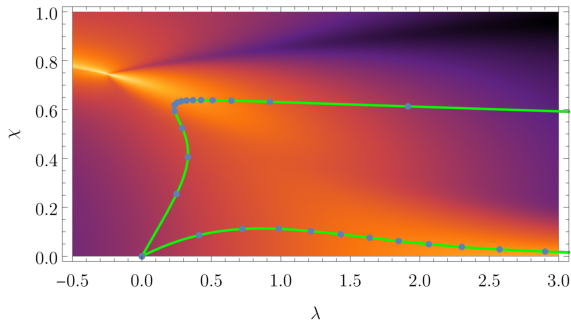
\includegraphics[scale=1.2]{../img/bg123.pdf}
    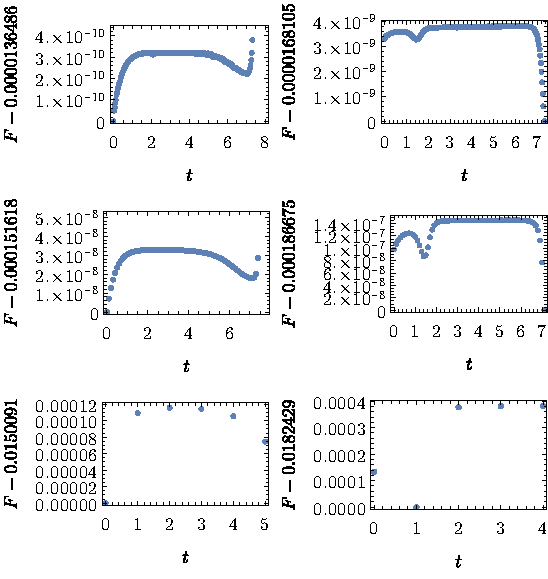
\includegraphics[scale=0.6]{../img/plotsFidelityQuenches.pdf}
    \caption{Fidelity for sequential quenches along geodesics (see green lines on top). Left (right) column corresponds to lower (upper) geodesic. Time steps from top are $\Delta t\in \{0.03,0.1,0.5\}$. Time difference between points in the plot on top is $\Delta t=0.5$.}
    \label{fig:plotsFidelityQuenches}    
\end{figure}



